\documentclass[journal,letterpaper,twoside,twocolumn]{IEEEtran}

\usepackage{graphicx}
\usepackage[spanish]{babel}
\usepackage[utf8]{inputenc}
\usepackage[T1]{fontenc}
\usepackage{cite}

\graphicspath{{../images/}{./images/}}% pdflatex must be compiled from bin directory to mantain a clean repo 
\newcommand{\myreferences}{../../../doc/review/review/library}% SPECIFY THIS PATH!!!
\bibliographystyle{IEEEtran}% apsr, agsm, dcu, kluwer, nederlands

\title{Locomoción Humanoide:\\Contacto, Impacto y Dinámica Centroidal}
\author{Jaime Andrés~Castillo-León}
\markboth{Primer Artículo: Métodos de Simulación en Física}{Castillo-León: Locomoción Humanoide}

\begin{document}
\maketitle
\begin{abstract}
  En este documento se propone trabajar con dinámica multicuerpo, aplicada a una configuración humanoide utilizando el formalismo de los screws para describir la dínamica del centro de masa y el momento angular del sistema. La interacción con el entorno será llevada a cabo por el impacto y contacto de los pies, cuyo modelo será propuesto a partir de esferas.
\end{abstract}
\begin{IEEEkeywords}
  Locomoción humanoide, Modelos de Impacto y Contacto, Dinamica Centroidal, Screws
\end{IEEEkeywords}

\section{Introducción}
\label{sec:intro}
\IEEEPARstart{P}{arte} de los problemas actuales de la simulación de la locomóción humanoide y sus aplicaciones a la biomecánica y las neurociencias, radíca en que los modelos de contacto y fricción actuales difieren bastante de la realidad\cite{Todorov2014}. Además la forma adecuada en que se describen y analizan la dinámica de la estructuras mecánicas, ha sido un reto para generar simulaciones en tiempo real\cite{Wensing2016}. Se ha probado diferentes formalismos: desde la mecánica clásica de las ecuaciónes de Newton-Euler, la mecánica analitica de Euler-Lagrange, los sistemas multipuertos de los Hamitonianos utilizando Bond Graphs o las ecuaciones de Kane partiendo del concepto de trabajo virtual. 

Generalmente cuando se utiliza el formalismo de Newton-Euler, para resolver la mecánica de cadenas cinemáticas tipo árbol, como las que se presentan en el cuerpo de los animales o en general de los seres vivos. Se debe plantear por cada cuerpo o eslabón que constituye a la cadena, seis ecuaciones de movimiento y luego se debe colocar restricciónes algebraicas para representar la física de las articulaciones, que finalmente representa la topología del mecanismo\cite{Taga1991}. Un motor físico, empleado para video juegos, ODE\cite{Smith2007}, soluciona las ecuaciones de movimiento, colision y friccion de esta forma, generando demasiadas ecuaciones. Se ha demostrado en varios artículos mediante benchmarks\cite{Sherman2011a,Erez2015} que este enfoque no es el adecuado para el análisis la locomoción de seres vivos\cite{Geijtenbeek2013,Wensing2015}.

Las ecuaciones de Euler-Lagrange producen un sistema de ecuaciones reducido, representado por variables generalizadas\cite{Spong2006}. A diferencia de Newton-Euler, el sistema a resolver es pequeño, lo cual para la síntesis de controladores es ventajoso a nivel computacional, no obstante este formalismo basado en el lagrangiano del sistema, no permite obtener de forma directa las fuerzas de interacción entre los cuerpos, las cuales son un requerimiento para el diseño mecánico del sistema. La topología de la cadena queda absorbida en el planteamiento del problema\cite{Featherstone2005}. Básicamente estos sistemas requiere de un motor algebraico diferencial para su solución, este motor se ejecuta como un preproceso y si la topología cambia se debe repetir el proceso\cite{Docquier2013}, situacion que no ocurre por Newton-Euler.

En el caso de los puertos Hamiltonianos, por ejemplo los Bond Graphs, representan un método gráfico para describir el flujo de energía del sistema, mediante dos variables: flujo y esfuerzo, además de la causalidad del sistema\cite{VanderSchaft2014}. La causalidad en este formalismo es utilizada para la implementación computacional automática de cómo deben ser planteadas y resueltas la ecuaciones de movimiento\cite{damic2015,Nageshrao2015b}. Una ventaja de los Bond Graphs es la aprarente sencilles con la que se puede acomplar diferentes medios físicos con el uso de los puertos, de allí que estos métodos se utilicen para problemas que involucran varios dominios físicos, como transferencia de calor, de masa, electromagnetismo y mecánica\cite{Nageshrao2015b}.

En este trabajo se propone utilizar un formalismo que puede moverse entre los cuatro anteriormente mencionados. Las ecuaciones de Lagrange son obtenidas a partir de algoritmos recursivos de Newton-Euler que a su vez son implementados utlizando el algebra de los Screws. Del sistema descrito en lagrangianos es posible obtener su representación en hamiltonianos y la construcción de las ecuaciones de Kane\cite{Liu2005a}. Los Screws permiten plantear las ecuaciones de movimiento de una forma más compacta y general, en donde se unen la translación y la rotación en una unica entidad matemática denomiada Screw\cite{Stramigioli2001}. La notación y construcción que se utilizará es la propuesta por Roy Feathrestone, en donde los Screws son definidos \emph{Vectores Espaciales} o \emph{6D-vectors}, con su respectiva algebra\cite{Featherstone2008,Featherstone2010b,Featherstone2010a}. Basicamente se definen dos tipos de Espacios Vectoriales: movimiento \emph{(Twist)} y fuerza \emph{(Wrenches)}\cite{Featherstone2006}.

Una vez son obtenidas las ecuaciones de movimiento por cualquier método, se debe resolver las ecuaciones diferenciales. Éstas ecuaciones requieren que el solucionador tenga dos propiedades: (1) control de tamaño de paso adaptativo, para controlar el error y (2) resolver ecuaciones numéricamente rígidas (\emph{stiff}). Para esto las librerias Odeint\cite{Ahnert2011} de Boost desarrolladas bajo el paradigma de metaprogramación presente C++ fueron utilizadas. Para la dinámica multicuerpo, se requiere de solucionar cadenas cinemáticas interconectadas mediante articulaciones de varios grados de libertad, la libreria RBDL\cite{Felis2016} en C++, implementa el trabajo de\cite{Featherstone2008}, para resolver el problema de la \emph{dinamica directa}, bajo un algoritmo de complejidad lineal en tiempo y espacio.

\section{Simulación Multicuerpo}
\label{sec:simula}
El modelo del humanoide (ver Figura.\ref{fig:humModel}), consta de una cadena cinemática tipo árbol con base flotante ubicada en la pelvis, representada por la esfera parcialmente visible de color morado. La pelvis representa una articulación de cuerpo libre con 6 grados de libertad. Las esferas de color azul claro o \emph{cyan}, representan las articulaciones restantes. En los hombros, el cuello, las caderas y la zona lumbar de la columna, se encuentra un total de seis articulaciones esféricas. Los cilindros de color cyan, representan articulaciones rotacionales de uno o dos ejes perpendiculares. Las muñecas y los tobillos representan articulaciones de dos grados de libertad. Finalmente las rodillas y codos tiene un grado rotacional. Esta configuración humanoide suma un total de 34 grados de libertad. Los algoritmos de Featherstone para la solución de la dínámica multicuerpo, en particular el algoritmo recursivo de \emph{cuerpos articulados}, con complejidad $\mathcal{O}(n)$ y $n$ los grados de libertad es empleado para solucionar la dinamica directa del humanoide.
\begin{figure}[!t]
  \centering
  \includegraphics[scale=0.5]{Whole-Body.png}
  \caption{Modelo humanoide}
  \label{fig:humModel}
\end{figure}

Debido a que el modelo está embebido en el espacio tridimensional, el uso de cuaterniones para la articulación de la pelvis es necesario para evitar cualquier tipo de singularidad. Las articulaciones esféricas también pueden requerir de el uso de cuaterniones para evitar inestabilidades númericas en las cercanias de las singularidades. La implicación del uso de cuaterniones se ve reflejado en los esquemas de integración de las ecuaciones, que pasan de ser ecuaciones diferenciales ordinarias a ecuaciones diferenciales algebraicas. El método de Euler es el método utilizado en este trabajo. Lo que implica perder las capacidades adaptativas y de rigidez de los otros métodos ya mensionados.

Los parámetros de centros de masa, tensores de inercia, longitudes y masas fueron tomados de \cite{Leva1996}. Las configuraciones de las articulaciónes fueron asumidas en este artículo.  

Para la simulación se utilizó un scipt descriptivo del humanoide en LUA, que puede ser fácilmente generado y leído por las liberías de RBDL. El mismo script descriptivo es utilzado por un visualizador basado en openGL y Qt, denominado MeshUp desarrollado por Martin Felis. El código generado para este articulo genera un archivo de CSV con la evolucion del tiempo y las articualaciones del sistema. 

\section{Modelos de Impacto y Contacto}
\label{sec:impYcon}
El modelo de fricción es una extensión del model de Hertz, utilizando el resorte de Cundall. Incluye el modelo de fricción de Coulomb y efectos visco-elasticos sobre el cual se puede analizar la perdida de energía en el sistema. El pie se modela como se ilustra en la Figura \ref{fig:humModel} y según se propuson en \cite{Felis2016a} (ver Figura \ref{fig:footModel}). 
\begin{figure}[!h]
  \centering
  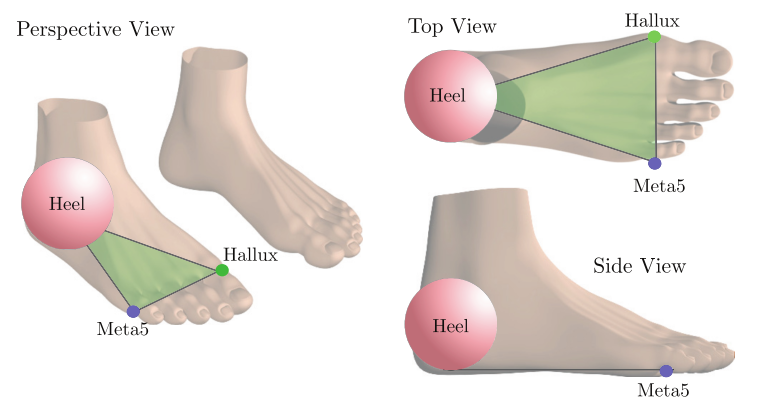
\includegraphics[scale=0.3]{Felis2016aFeetModel.png}
  \caption{Modelo del pie para el contacto y la colisión \protect\cite{Felis2016a}.}
  \label{fig:footModel}
\end{figure}

Para el modelo humanoide completo se propuso, un sistema de esferas que pudiera colisionar con el entorno. Cada esfera pertenecia a un único eslabón de la cadena cinemática. Las fuerzas producidas por el modelo de Hertz, son utilizadas como entrada en los algoritmos de dinamica directa del humanoide. Las fuerzas producidas en las esferas están representadas en un marco de referncia global y deben ser llebadas a un marco de referencia local a cada eslabón para aprovechar las virtudes del algoritmo de \emph{cuerpos articulados}.

El sistema de colisiones se puede ver en la figura \ref{fig:CollisionModel}, todas las esferas menos las amarillas son esferas conectadas a un único eslabón, sobre el cual se debe solucionar un equilibrio dinámico. Se realizo pruebas de simetría y validación del modelo de friccíon y la integración con las librerias utilizando solo esferas. Posterior a esto se colocó la arquitectura del humanoide en una posición simétrica y se dejo caer por acción de la gravedad. 
\begin{figure}[!h]
  \centering
  \includegraphics[scale=0.3]{CollisionSystem.png}
  \caption{Sistema de colisiones.}
  \label{fig:CollisionModel}
\end{figure}

El principal experimento, figura \ref{fig:Bruces}, fue dejar caer el humanoide desde una altura de 1.2 metros de la cadera al piso por acción de la gravedad, con una inclinación de 30 grados con respecto al plano horizontal. La figura muestra la evolución de cada uno de los marcos de referncia de cada eslabón. La escala de tiempo esta representada en mapa de color tipo JET. El color azul oscuro parte del tiempo 0 segundos y el color rojo tiende al segundo 5 de la caída, los colores verdes y amarillos son tiempos intermedios. El sub-recuadro de borde negro, enfatiza oscilaciones no coherentes con la realidad al utilizar el resorte de Cundall. Esta oscilaciones no presentan al remover las fuerzas tangenciales de dicho modelo. 
\begin{figure}[!h]
  \centering
  \includegraphics[scale=0.4]{CaerDeBruces.png}
  \caption{Caída de bruces.}
  \label{fig:Bruces}
\end{figure}

\section{Discusión y Conclusiones}
\label{sec:conclu}
\emph{Desventajas:} (1) Los ajustes de los parámetros visco-elástico del modelo, se realizan de forma manual mediante ensayo y error. (2) Los tiempos de integración maximos son de 0.0001 segundos, lo cual es 100 veces más pequeño que un simulador utilizando otro tipo de modelo de colisión\cite{Todorov2014}. (3) Los resultados obtenidos por el efecto del resorte de Cundall produce comportamiento oscilantes sobre las superficies que no son apreciables en la realidad.

\emph{Ventajas:} (1) Finalmente se produjo una estructura de código orientado a objetos, modular sobre el cual se puede probar diferentes integradores, modelos de colision y fricción.


\bibliography{\myreferences}

\end{document}
